\begin{center}
\LARGE
Delprøve uden hjælpemidler 
\end{center}
\stepcounter{section}
%%%%%%%%%%%%%%%%%%%%%%%%%%%%%%%%%%%%%%%%%%%%%%%%%%%%%%%%%%%%%%%%%%%%%%%
%							Ny Opgave!!!!!							%
%%%%%%%%%%%%%%%%%%%%%%%%%%%%%%%%%%%%%%%%%%%%%%%%%%%%%%%%%%%%%%%%%%%%%%%
\begin{opgavetekst}{Opgave 1}
\end{opgavetekst}
	\begin{delopgave}{}{1}
		Løs ligningen 
		\begin{align*}
			7(x-5) = 12x-10
		\end{align*}
	\end{delopgave}
%%%%%%%%%%%%%%%%%%%%%%%%%%%%%%%%%%%%%%%%%%%%%%%%%%%%%%%%%%%%%%%%%%%%%%%
%							Ny Opgave!!!!!							%
%%%%%%%%%%%%%%%%%%%%%%%%%%%%%%%%%%%%%%%%%%%%%%%%%%%%%%%%%%%%%%%%%%%%%%%
\begin{opgavetekst}{Opgave 2}
\end{opgavetekst}
	\begin{delopgave}{}{1}
		Reducér udtrykket 
		\begin{align*}
			 \frac{(a^3+b)ab^2-a^4b^2}{b^2}
		\end{align*}
	\end{delopgave}
%%%%%%%%%%%%%%%%%%%%%%%%%%%%%%%%%%%%%%%%%%%%%%%%%%%%%%%%%%%%%%%%%%%%%%%
%							Ny Opgave!!!!!							%
%%%%%%%%%%%%%%%%%%%%%%%%%%%%%%%%%%%%%%%%%%%%%%%%%%%%%%%%%%%%%%%%%%%%%%%
\begin{opgavetekst}{Opgave 3}
	En linje $l$ går gennem punktet $(1,-2)$ og har normalvektoren
	\begin{align*}
		\vv{n} = 
		\begin{pmatrix}
			3 \\ 4
		\end{pmatrix}.
	\end{align*}	
\end{opgavetekst}
\begin{delopgave}{}{1}
	Bestem linjens ligning for $l$. 
\end{delopgave}
\begin{meretekst}
	En linje $m$ er bestemt ved ligningen
	\begin{align*}
		y = 2x+7
	\end{align*}
\end{meretekst}
\begin{delopgave}{}{2}
	Bestem skæringspunktet mellem $l$ og $m$.
\end{delopgave}
%%%%%%%%%%%%%%%%%%%%%%%%%%%%%%%%%%%%%%%%%%%%%%%%%%%%%%%%%%%%%%%%%%%%%%%
%							Ny Opgave!!!!!							%
%%%%%%%%%%%%%%%%%%%%%%%%%%%%%%%%%%%%%%%%%%%%%%%%%%%%%%%%%%%%%%%%%%%%%%%
\begin{opgavetekst}{Opgave 4}
	Et tredjegradspolynomium $f$ er givet ved
	\begin{align*}
		f(x) = (x-1)(x^2-x-12).
	\end{align*}
\end{opgavetekst}
\begin{delopgave}{}{1}
	Bestem $f(2)$.
\end{delopgave}
\begin{delopgave}{}{2}
	Bestem rødderne for $f$. 
\end{delopgave}
%%%%%%%%%%%%%%%%%%%%%%%%%%%%%%%%%%%%%%%%%%%%%%%%%%%%%%%%%%%%%%%%%%%%%%%
%							Ny Opgave!!!!!							%
%%%%%%%%%%%%%%%%%%%%%%%%%%%%%%%%%%%%%%%%%%%%%%%%%%%%%%%%%%%%%%%%%%%%%%%
\newpage
\begin{opgavetekst}{Opgave 5}
	En cirkel $C$ har centrum i $(3,-4)$ og radius $5$.
\end{opgavetekst}
\begin{delopgave}{}{1}
	Opskriv en ligning for $C$.
\end{delopgave}
\begin{delopgave}{}{2}
	Brug dit svar på a) til at afgøre, om punktet $(3,1)$ ligger på $C$.
\end{delopgave}
%%%%%%%%%%%%%%%%%%%%%%%%%%%%%%%%%%%%%%%%%%%%%%%%%%%%%%%%%%%%%%%%%%%%%%%
%							Ny Opgave!!!!!							%
%%%%%%%%%%%%%%%%%%%%%%%%%%%%%%%%%%%%%%%%%%%%%%%%%%%%%%%%%%%%%%%%%%%%%%%
\begin{opgavetekst}{Opgave 6}
	En linje $l$ er givet ved
	\begin{align*}
		l: \ 3x -4y + 6 = 0,
	\end{align*}
	og et punkt $P$ er givet ved $P(2,-2)$.
\end{opgavetekst}
\begin{delopgave}{}{1}
	Bestem den korteste afstand fra $l$ til $P$. 
\end{delopgave}
\newpage
\begin{center}
\LARGE
Delprøve med hjælpemidler 
\end{center}
\stepcounter{section}
%%%%%%%%%%%%%%%%%%%%%%%%%%%%%%%%%%%%%%%%%%%%%%%%%%%%%%%%%%%%%%%%%%%%%%%
%							Ny Opgave!!!!!							%
%%%%%%%%%%%%%%%%%%%%%%%%%%%%%%%%%%%%%%%%%%%%%%%%%%%%%%%%%%%%%%%%%%%%%%%
\begin{opgavetekst}{Opgave 7}
	\begin{center}
		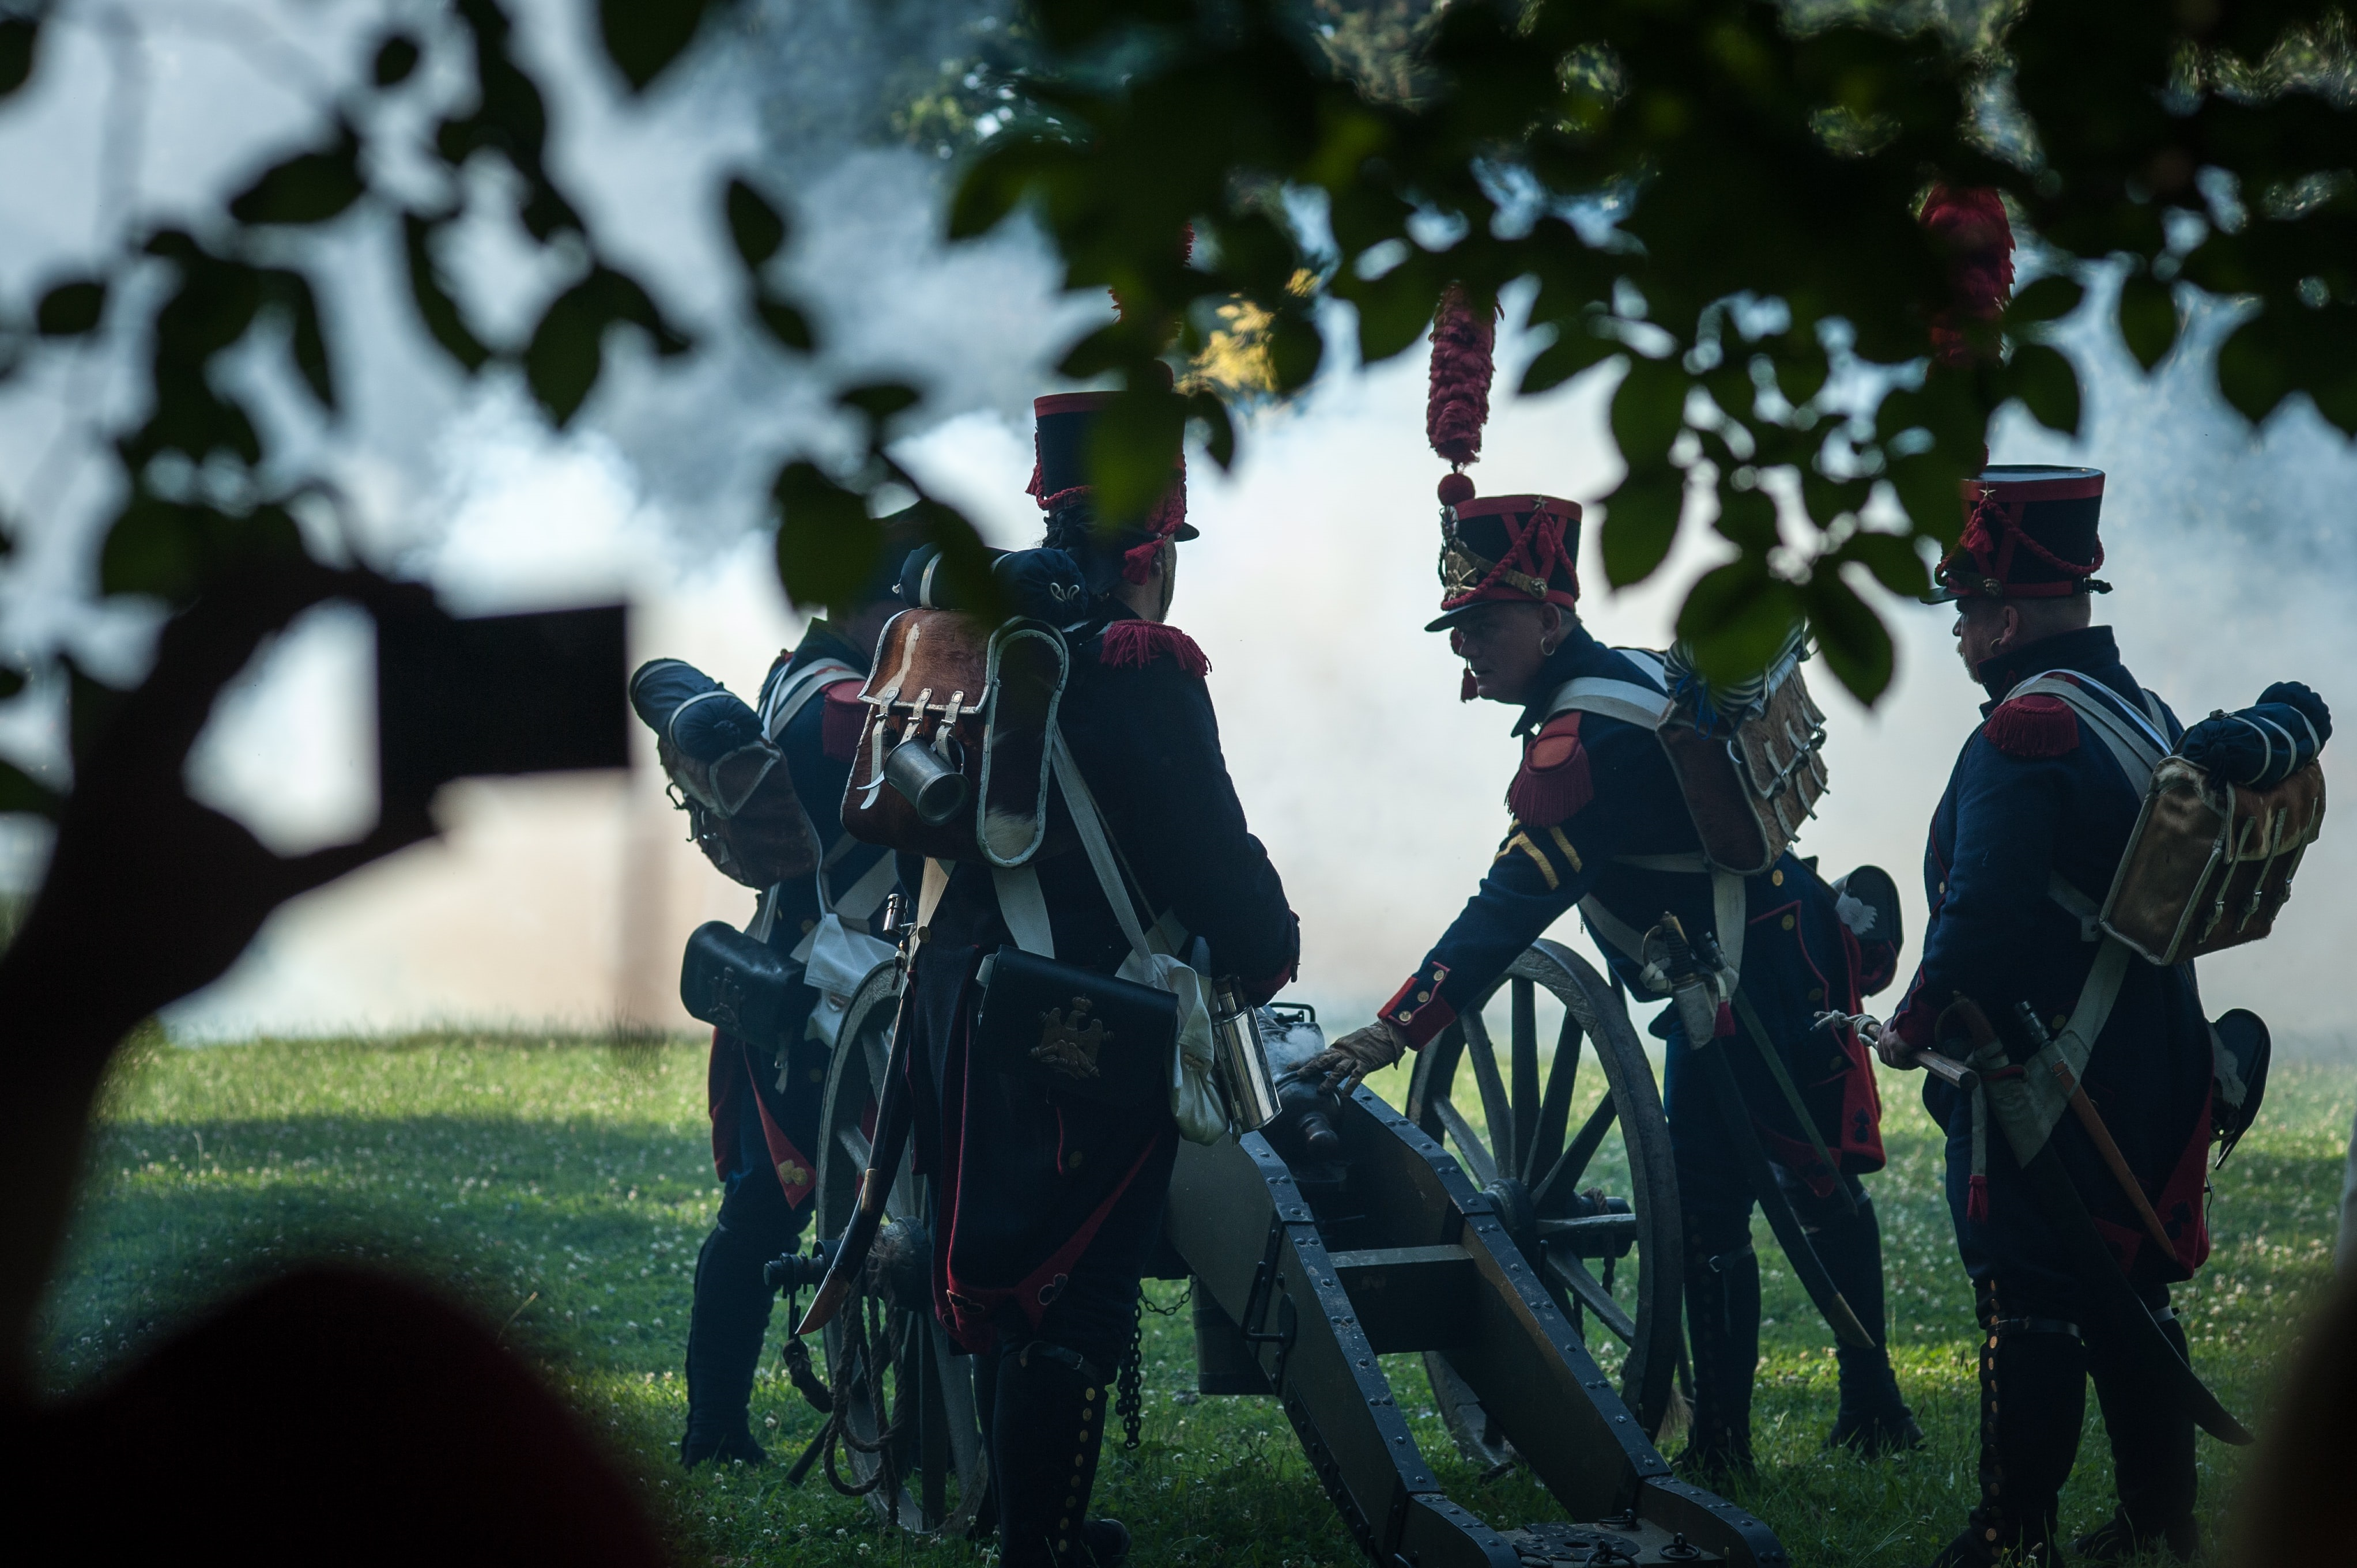
\includegraphics[width=0.6\textwidth]{Billeder/kanon.jpg}
	\end{center}
	Under den 2. Slesviske krig skulle de østrigske og preussiske kanoner skyde over Vemmingbund for at ramme de danske skanser ved Dybbøl mølle. Skudafstanden afhænger af affyringsvinklen på kanonen
	og for at skyde den rigtige afstand er det vigtigt at kende den korrekte affyringsvinkel. Af Tab.  \ref{tab:kanon} kan sammenhængen mellem affyringsvinklen $x$ (i grader) og skudafstanden $D$
	(i meter) ses.
	\begin{table}[H]
		\centering
		\begin{tabular}{c|c|c|c|c|c|c|c}
		$x$ &10 & 20 & 30 & 40 & 50 & 60 & 70 \\
		\hline
		$D$ & 1197 & 2089 & 2655 & 2968 & 3022 & 2659 & 2082
		\end{tabular}
		\caption{Sammenhæng mellem skudafstand (i meter) og affyringsvinkel (i grader)}
		\label{tab:kanon}
	\end{table}\phantom{h}
	En model for affyringsafstanden $D$ som funktion af affyringsvinklen $x$ er givet ved
	\begin{align*}
		D(x) = ax^2+bx+c
	\end{align*}
\end{opgavetekst}
\begin{delopgave}{}{1}
	Brug tallende fra Tab. \ref{tab:kanon} til at bestemme en forskrift for $D$.
\end{delopgave}
\begin{delopgave}{}{2}
	Hvor langt skyder kanonen, hvis affyringsvinklen er $25^\circ$?
\end{delopgave}
\begin{meretekst}
	Det oplyses, at der er $1.8$km fra de preussisk/østrigske skanser til Skanse 1 ved Vemmingbund. 
\end{meretekst}
\begin{delopgave}{}{3}
	Hvilken affyringsvinkel skal bruges for at ramme Skanse 1?
\end{delopgave}
%%%%%%%%%%%%%%%%%%%%%%%%%%%%%%%%%%%%%%%%%%%%%%%%%%%%%%%%%%%%%%%%%%%%%%%
%							Ny Opgave!!!!!							%
%%%%%%%%%%%%%%%%%%%%%%%%%%%%%%%%%%%%%%%%%%%%%%%%%%%%%%%%%%%%%%%%%%%%%%%
\newpage
\begin{opgavetekst}{Opgave 8}
	En cirkel $C$ er givet ved ligningen 
	\begin{align*}
		C: \ x^2-6x+y^2-10y=30
	\end{align*}
\end{opgavetekst}
\begin{delopgave}{}{1}
	Bestem centrum og radius for $C$.
\end{delopgave}
\begin{meretekst}
	En linje $l$ er givet ved ligningen 
	\begin{align*}
		l: \ y = -2x+5.
	\end{align*}
\end{meretekst}
\begin{delopgave}{}{2}
	Bestem skæringspunkterne $P$ og $Q$ mellem $l$ og $C$. 
\end{delopgave}
\begin{delopgave}{}{3}
	Bestem en ligning for tangenten til cirklen i både $P$ og $Q$.
\end{delopgave}
